% Homework template for Information Theory and Statistical Learning
% by Xiangxiang Xu <xiangxiangxu.thu@gmail.com>
% LAST UPDATE: Oct 3, 2019
\documentclass[a4paper]{article}
\usepackage[T1]{fontenc}
\usepackage{amsmath, amssymb, amsthm}
% amsmath: equation*, amssymb: mathbb, amsthm: proof
\usepackage{moreenum}
\usepackage{mathtools}
\usepackage{url}
\usepackage{enumitem}
\usepackage{bm}
\usepackage{graphicx}
\usepackage{subcaption}
\usepackage{booktabs} % toprule
\usepackage[mathcal]{eucal}
\usepackage{dsfont}
\usepackage[numbered,framed]{matlab-prettifier}
%% Definitions for Information Theory & Statistical Learning
%% UPDATED: Sep 30, 2019 by Xiangxiang 
\newcommand{\theterm}{Fall 2020}

\newcommand{\thecoursenameshort}{\textsc{Information Theory and Statistical Learning}}
\newcommand{\thecoursename}{
Tsinghua-Berkeley Shenzhen Institute\\
%\vspace*{0.1in}
\thecoursenameshort
}

\newcommand{\courseheader}{
\vspace*{-1in}
\begin{center}
\thecoursename \\
\theterm
\vspace*{0.1in}
\hrule
\end{center}
}
\newcommand{\uc}{\underline{c}}    % c, vec
\newcommand{\uv}{\underline{v}}    % x, vec
\newcommand{\uw}{\underline{w}}    % w, vec
\newcommand{\ux}{\underline{x}}    % x, vec
\newcommand{\uy}{\underline{y}}    % y, vec
\newcommand{\uz}{\underline{z}}    % z, vec
\newcommand{\um}{\underline{m}}    % m, vec
\newcommand{\ut}{\underline{t}}    % t, vec

\newcommand{\bA}{\mathbf{A}}    % A, mat
\newcommand{\bI}{\mathbf{I}}    % A, mat
\newcommand{\bN}{\mathbf{N}}    % n, mat
\newcommand{\bT}{\mathbf{T}}    % T, mat
\newcommand{\bU}{\mathbf{U}}    % U, mat
\newcommand{\bV}{\mathbf{V}}    % V, mat
\newcommand{\bQ}{\mathbf{Q}}    % Q, mat
\newcommand{\bX}{\mathbf{X}}    % X, mat

\newcommand{\bc}{\bm{c}}    % c, vec
\newcommand{\be}{\bm{e}}    % e, vec
\newcommand{\bu}{\bm{u}}    % u, vec
\newcommand{\bv}{\bm{v}}    % v, vec
\newcommand{\bw}{\bm{w}}    % w, vec
\newcommand{\bt}{\bm{t}}    % t, vec
\newcommand{\bx}{\bm{x}}    % x, vec
\newcommand{\by}{\bm{y}}    % y, vec
\newcommand{\bz}{\bm{z}}    % z, vec

\newcommand{\phib}{\bm{\phi}}    % phi, vec
\newcommand{\psib}{\bm{\psi}}    % psi, vec
\newcommand{\dtm}{\mathbf{B}}    %
\newcommand{\dtmt}{\tilde{\dtm}}    %
\newcommand{\Ab}{\mathbf{A}}    % A mat
\newcommand{\Kb}{\mathbf{K}}    % K mat
\newcommand{\Ib}{\mathbf{I}}    % I mat



\newcommand{\rvby}{\bm{\mathsf{y}}}    % y, rv. vec
\newcommand{\rvbx}{\bm{\mathsf{x}}}    % x, rv. vec
% \newcommand{\bm}{\bm{m}}    % m, vec
\newcommand{\bzero}{\bm{0}}    % 0, vec

\newcommand{\balpha}{\bm{\alpha}}    % alpha, vec
\newcommand{\bphi}{\bm{\phi}}    % phi, vec
\newcommand{\bpsi}{\bm{\psi}}    % psi, vec
\newcommand{\bxi}{\bm{\xi}}    % xi, vec
\newcommand{\btheta}{\bm{\theta}}    % theta, vec
\newcommand{\bmu}{\bm{\mu}}    % mu, vec

\newcommand{\bLambda}{\bm{\Lambda}}    % Sigma, mat
\newcommand{\bSigma}{\bm{\Sigma}}    % Sigma, mat

\newcommand{\cF}{\mathcal{F}}  
\newcommand{\cL}{\mathcal{L}}  
\newcommand{\cX}{\mathcal{X}}  
\newcommand{\cY}{\mathcal{Y}}  

\newcommand{\rvx}{\mathsf{x}}    % x, r.v.
\newcommand{\rvy}{\mathsf{y}}    % y, r.v.
\newcommand{\rvz}{\mathsf{z}}    % z, r.v.
\newcommand{\rvw}{\mathsf{w}}    % w, r.v.
\newcommand{\rvv}{\mathsf{v}}    % v, r.v.
\newcommand{\rvm}{\mathsf{m}}    % m, r.v.
\newcommand{\rvt}{\mathsf{t}}    % t, r.v.
\newcommand{\rvH}{\mathsf{H}}    % H, r.v.
\newcommand{\urvx}{\underline{\mathsf{x}}}    % x, r.v. vec
\newcommand{\urvy}{\underline{\mathsf{y}}}    % y, r.v. vec
\newcommand{\urvz}{\underline{\mathsf{z}}}    % z, r.v. vec
\newcommand{\urvw}{\underline{\mathsf{w}}}    % w, r.v. vec
\newcommand{\urvt}{\underline{\mathsf{t}}}    % t, r.v. vec


\newcommand{\defeq}{\triangleq} %\coloneqq
\newcommand{\reals}{\mathbb{R}}
\newcommand{\T}{\mathrm{T}}    % transpose
\newcommand{\F}{\mathrm{F}}    % Frobenius
\newcommand{\BLS}{\mathrm{BLS}}    % BLS
\newcommand{\LLS}{\mathrm{LLS}}    % LLS
\newcommand{\MVU}{\mathrm{MVU}}    % MVU
\newcommand{\dd}{\mathrm{d}}  

\DeclareMathOperator*{\maximize}{maximize}    % maximize
\DeclareMathOperator*{\minimize}{minimize}    % minimize
\newcommand{\st}{\mathrm{subject~to}}    % minimize

% \newcommand{\E}[1]{\mathbb{E}\left[{#1}\right]}
% \newcommand{\Prob}[1]{\mathbb{P}\left({#1}\right)}
\DeclareMathOperator*{\argmax}{arg\,max}
\DeclareMathOperator*{\argmin}{arg\,min}
\DeclareMathOperator*{\argsup}{arg\,sup}
\DeclareMathOperator*{\arginf}{arg\,inf}
\DeclareMathOperator{\diag}{diag}
\DeclareMathOperator{\tr}{tr}
\DeclareMathOperator{\Cov}{Cov}
\DeclareMathOperator{\var}{var}
\DeclareMathOperator{\cov}{cov}
\DeclareMathOperator{\MSE}{MSE}
\DeclareMathOperator{\1}{\mathds{1}} % dsfont required
\DeclareMathOperator{\E}{\mathbb{E}}
\DeclareMathOperator{\Prob}{\mathbb{P}}
\DeclareMathOperator{\im}{im}
\DeclareMathOperator{\rank}{rank}
\DeclareMathOperator{\Bern}{Bern}
\DeclareMathOperator{\Binom}{Binom}

\newcommand\independent{\protect\mathpalette{\protect\independenT}{\perp}}
\def\independenT#1#2{\mathrel{\rlap{$#1#2$}\mkern2mu{#1#2}}}

%%% Local Variables:
%%% mode: latex
%%% TeX-master: "ithw"
%%% End:


\lstset{
  style              = Matlab-editor,
  captionpos         =b,
  basicstyle         = \mlttfamily,
  escapechar         = ",
  mlshowsectionrules = true,
}
\begin{document}
\courseheader



\newcounter{hwcnt}
\setcounter{hwcnt}{2} % set to the times of Homework

\begin{center}
  \underline{\bf Homework \thehwcnt} \\
\end{center}
\begin{flushleft}
  \textcolor{gray}{Hanmo Chen 2020214276}\hfill
  \today
\end{flushleft}
\hrule

\vspace{2em}
\setlist[enumerate,1]{label=\thehwcnt.\arabic*.}
\setlist[enumerate,2]{label=(\alph*)}
\setlist[enumerate,3]{label=\roman*.}
\setlist[enumerate,4]{label=\greek*)}

\flushleft
\rule{\textwidth}{1pt}
\begin{itemize}
\item {\bf Acknowledgments: \/} 

  For the Gamma function and its series extensions, I refer to the website(\url{https://www.wolframalpha.com/}). And for the proof of Karamata's Inequality, I refer to the wikipedia(\url{https://en.wikipedia.org/wiki/Karamata's_inequality}). Some matrix tricks used in deriviation comes from the Matrix Cookbook(\url{http://matrixcookbook.com/})
\item {\bf Collaborators: \/}
  \textcolor{gray}{None}

\item  \emph{I certify that all solutions are entirely in my words and that I have not looked at another student's solutions. I have credited all external sources in this write up.}
  \framebox[\linewidth]{\rule{0pt}{10pt}\textcolor{gray}{\large Hanmo Chen}}
\end{itemize}
\rule{\textwidth}{1pt}


\vspace{2em}


\begin{enumerate}
  \setlength{\itemsep}{3\parskip}

  \item First, we have Chain Rule for mutual information 
  
  \begin{equation}
    \begin{aligned}
      I\left(X_{1}, X_{2}, \cdots, X_{n} ; Y\right)&=\sum_{i=1}^{n} I\left(X_{i} ; Y \mid X_{i-1}, X_{i-2}, \cdots, X_{1}\right) \\
      I\left(X ; Y_1,Y_2,\cdots,Y_n \right)&=\sum_{i=1}^{n} I\left(X ; Y_i \mid Y_{i-1}, Y_{i-2}, \cdots, Y_{1}\right) 
    \end{aligned}
  \end{equation}

  Using this Chain Rule twice,

  \begin{equation}
    \begin{aligned}
      I\left(X_{1}, \ldots, X_{n} ; Y_{1}, \ldots, Y_{m}\right) & = \sum_{j=1}^m I\left(X_{1}, X_{2}, \cdots, X_{n} ; Y_j \mid Y_{j-1}, Y_{j-2}, \cdots, Y_{1}\right)  \\ 
      & = \sum_{i=1}^n \sum_{j=1}^m I\left(X_{i} ; Y_j \mid X_{i-1}, X_{i-2}, \cdots, X_{1},Y_{j-1}, Y_{j-2}, \cdots, Y_{1}\right)
    \end{aligned}
  \end{equation}


  \item Examples:
  \begin{enumerate}
    \item $I(X ; Y \mid Z)<I(X ; Y)$
    
        Let $Z=X$ then $I(X;Y\mid Z) = H(X\mid Z) - H(X,Y\mid Z) = 0$. But for $X,Y$ that are not independent, $I(X;Y)>0 = I(X ; Y \mid Z)$

    \item $I(X ; Y \mid Z)>I(X ; Y) $
    
      Use the example illustrated in class. let $X$ and $Y$ be independent Bernoulli random variables with $p=0.5 $, and let $Z = X+Y$. Then $I (X ; Y) = 0$, but $I (X ; Y | Z) = H(X | Z) - H(X | Y, Z) = H(X | Z) =  0.5$ bit.

  \end{enumerate}

  \item \textit{Information Measures.}
    \begin{enumerate}
      \item Denote $n=|A|$, because $Z_1,Z_2,\cdots,Z_n$ are i.i.d Bern$(\frac 1 2)$ random variables, so $X_A = (Z_i)_{i\in A}$ is a $n$-dimension random vector having $2^n$ possible points with equal probability, 
      \begin{equation}
        H(X_A) = 2^n *(-\frac 1 {2^n} \log \frac 1 {2^n}) = n = |A| ~\text{(bits)}
      \end{equation} 


      \item Denote $A = A_1 \cup A_2 , A^* = A_1 \cap A_2 ,A_1^* = A_1 \backslash A_2, A_2^* = A_2 \backslash A_1$, so $X_{A_1} = (X_{A^*},X_{A_1^*}),X_{A_2} = (X_{A^*},X_{A_2^*}) $. Because  $X_{A^*},X_{A_1^*},X_{A_2^*}$ are mutually independent,
      \begin{equation}
        \begin{aligned}
          H(X_{A_1}|X_{A_2}) & = H((X_{A^*},X_{A_1^*})|(X_{A^*},X_{A_2^*}) ) \\
          & = H(X_{A_1^*}) = |A_1^*| = |A_1 \backslash A_2|
        \end{aligned}
      \end{equation}

      Thus,

      \begin{equation}
        \begin{aligned}
          H(X_{A_1},X_{A_2}) & = H(X_{A_2}) + H(X_{A_1}|X_{A_2})  \\
          & =  |A_2| + |A_1^*| = |A_1 \cup A_2|
        \end{aligned}
      \end{equation}

      \begin{equation}
        \begin{aligned}
          I(X_{A_1};X_{A_2}) & = H(X_{A_2}) - H(X_{A_2}|X_{A_1})  \\
          & =  |A_2| - |A_2^*| = |A_1 \cap A_2|
        \end{aligned}
      \end{equation}

    \end{enumerate}


    \item 
    \begin{enumerate}
    \item No. $f_{X,Y}(x,y) = 0.5,|x|+|y|\leqslant 1$, and $f_X(x) = 1-|x|,x\in [-1,1],f_Y(y) = 1-|y|,y\in [-1,1]$, $f_{X,Y}(x,y) \neq f_X(x)f_Y(y)$ so $X,Y$ are not independent. 
    \item  Because $X$ and $Y$ are symmetric, $H(X)=H(Y)$ and $I(X;Y) = H(X)+H(Y)-H(X,Y) = 2H(X)-H(X,Y)$. 
    
    Denote the area of $B_p$ as $S_p = 4\int_{0}^{1} (1-|x|^p)^{1/p} dx $, 
    
    joint distribution of $(X,Y)$ is $f_p(x,y)= \frac{1}{S_p},|x|^{p}+|y|^{p} \leqslant 1$ 
    
    the \textit{pdf} of $X$ is $f_p(x) = \frac 2 {S_p} (1-|x|^p)^{1/p},x \in [-1,1]$

    So

    \begin{equation}
      I(X;Y) = 2H(X)-H(X,Y) = -2 \int_{-1}^1 f_p(x)\log(f_p(x)) dx -\log  S_p
    \end{equation}

    \begin{itemize}
      \item $p=\frac 1 2,S_p = \frac 2 3$, $I(X;Y) =\frac 7 3 -\ln3-\ln2 = 0.542$
      \item $p = 1,S_p = 2,I(X;Y) = 1 -\ln 2 = 0.307$
      \item $p = \infty$, $X,Y$ are independent, $I(X;Y) = 0$
    \end{itemize}

    \item \begin{equation}
      \lim_{p\to 0} I(X;Y) = \infty
    \end{equation}
    Denote $n = 1/p$,
    \begin{equation}
      S_p = 4\int_{0}^1 (1-x^{\frac 1 n})^n dx = 4n\int_{0}^1 t^n (1-t)^{n-1}dt  = 4 \frac {(\Gamma(n+1))^2}{\Gamma(2n+1)}
    \end{equation}

    And 

    \begin{equation}
      I_n(X;Y) = 2n(\sum_{i=n+1}^{2n} \frac 1 i)  - \log \frac {(2n)!}{(n!)^2}
    \end{equation}

    Because 

    \begin{equation}
      \lim_{n\to\infty} \sum_{i=n+1}^{2n} \frac 1 i  = \ln 2
    \end{equation}


    \begin{equation}
      \log \frac {(2n)!}{(n!)^2} = \log \left(\frac{2^{2 n} \Gamma\left(n+\frac{1}{2}\right)}{\Gamma(n+1)}\right)-\frac{\log (\pi)}{2}
    \end{equation}

    And $\frac{ \Gamma\left(n+\frac{1}{2}\right)}{\Gamma(n+1)} \sim \log(n)$ as $n\to\infty$, thus

    \begin{equation}
      \lim_{n\to \infty} I_n(X;Y) =  \lim_{n\to \infty} \frac 1 2 \log(n) =  \infty
    \end{equation}

    \end{enumerate}

    \item The density function of Gaussian distribution is 
    \begin{equation}
      p(\mathbf{x})=\frac{1}{(2 \pi)^{n / 2}|\Sigma|^{1 / 2}} \exp \left(-\frac{1}{2}(\mathbf{x}-\boldsymbol{m})^{T} \Sigma^{-1}(\mathbf{x}-\boldsymbol{m})\right)
    \end{equation}

    Thus, 
    \begin{equation}
      \begin{aligned}
        D\left(\mathcal{N}\left(\boldsymbol{m}_{1}, \boldsymbol{\Sigma}_{1}\right) \| \mathcal{N}\left(\boldsymbol{m}_{0}, \boldsymbol{\Sigma}_{0}\right)\right) & = \mathbb{E}_{\mathcal{N}\left(\boldsymbol{m}_{1}, \boldsymbol{\Sigma}_{1}\right)}[\log \left( \frac {p_1(\mathbf{x})}{p_0(\mathbf{x})}\right)] \\
        & =\mathbb{E}_{\mathcal{N}\left(\boldsymbol{m}_{1}, \boldsymbol{\Sigma}_{1}\right)}\Bigg[\frac{1}{2} \log \frac{\left|\boldsymbol{\Sigma}_{0}\right|}{\left|\boldsymbol{\Sigma}_{1}\right|}-\frac{1}{2}\left(\mathbf{x}-\boldsymbol{m}_{1}\right)^{T} \boldsymbol{\Sigma}_{1}^{-1}\left(\mathbf{x}-\boldsymbol{m}_{1}\right)\\ 
        &\quad+\frac{1}{2}\left(\mathbf{x}-\boldsymbol{m}_{0}\right)^{T} \boldsymbol{\Sigma}_{0}^{-1}\left(\mathbf{x}-\boldsymbol{m}_{0}\right)\Bigg] \\ 
        & =\frac{1}{2} \log \frac{\left|\boldsymbol{\Sigma}_{0}\right|}{\left|\boldsymbol{\Sigma}_{1}\right|}-\frac{1}{2} \mathbb{E}_{\mathcal{N}\left(\boldsymbol{m}_{1}, \boldsymbol{\Sigma}_{1}\right)}\left[\left(\mathbf{x}-\boldsymbol{m}_{1}\right)^{T} \boldsymbol{\Sigma}_{1}^{-1}\left(\mathbf{x}-\boldsymbol{m}_{1}\right)\right] \\
        & \quad +\frac{1}{2} \mathbb{E}_{\mathcal{N}\left(\boldsymbol{m}_{1}, \boldsymbol{\Sigma}_{1}\right)}\left[\left(\mathbf{x}-\boldsymbol{m}_{0}\right)^{T} \boldsymbol{\Sigma}_{0}^{-1}\left(\mathbf{x}-\boldsymbol{m}_{0}\right)\right]
      \end{aligned}
    \end{equation}

    For $\mathbb{E}_{\mathcal{N}\left(\boldsymbol{m}_{1}, \boldsymbol{\Sigma}_{1}\right)}\left[\left(\mathbf{x}-\boldsymbol{m}_{1}\right)^{T} \boldsymbol{\Sigma}_{1}^{-1}\left(\mathbf{x}-\boldsymbol{m}_{1}\right)\right]$,

    \begin{equation}
      \begin{aligned}
        \mathbb{E}_{\mathcal{N}\left(\boldsymbol{m}_{1}, \boldsymbol{\Sigma}_{1}\right)}\left[\left(\mathbf{x}-\boldsymbol{m}_{1}\right)^{T} \boldsymbol{\Sigma}_{1}^{-1}\left(\mathbf{x}-\boldsymbol{m}_{1}\right)\right] & = \text{tr}\left(\mathbb{E}_{\mathcal{N}\left(\boldsymbol{m}_{1}, \boldsymbol{\Sigma}_{1}\right)}\left[\left(\mathbf{x}-\boldsymbol{m}_{1}\right)^{T} \boldsymbol{\Sigma}_{1}^{-1}\left(\mathbf{x}-\boldsymbol{m}_{1}\right)\right]\right) \\
        & = \mathbb{E}_{\mathcal{N}\left(\boldsymbol{m}_{1}, \boldsymbol{\Sigma}_{1}\right)}\left[\text{tr}\left(\left(\mathbf{x}-\boldsymbol{m}_{1}\right)^{T} \boldsymbol{\Sigma}_{1}^{-1}\left(\mathbf{x}-\boldsymbol{m}_{1}\right)\right)\right] \\
        & = \mathbb{E}_{\mathcal{N}\left(\boldsymbol{m}_{1}, \boldsymbol{\Sigma}_{1}\right)}\left[\text{tr}\left(\left(\mathbf{x}-\boldsymbol{m}_{1}\right)\left(\mathbf{x}-\boldsymbol{m}_{1}\right)^{T} \boldsymbol{\Sigma}_{1}^{-1}\right)\right] \\
        & = \text{tr}\left(\mathbb{E}_{\mathcal{N}\left(\boldsymbol{m}_{1}, \boldsymbol{\Sigma}_{1}\right)}\left[\left(\mathbf{x}-\boldsymbol{m}_{1}\right)\left(\mathbf{x}-\boldsymbol{m}_{1}\right)^{T}\right] \boldsymbol{\Sigma}_{1}^{-1}\right) \\
        & = \text{tr}\left(\boldsymbol{\Sigma}_{1}\boldsymbol{\Sigma}_{1}^{-1}\right) = \text{tr}(\boldsymbol{I_n}) = n
      \end{aligned}
    \end{equation}

    In the same way, 

    \begin{equation}
      \begin{aligned}
        \mathbb{E}_{\mathcal{N}\left(\boldsymbol{m}_{1}, \boldsymbol{\Sigma}_{1}\right)}\left[\left(\mathbf{x}-\boldsymbol{m}_{0}\right)^{T} \boldsymbol{\Sigma}_{0}^{-1}\left(\mathbf{x}-\boldsymbol{m}_{0}\right)\right] & = \text{tr}\left(\mathbb{E}_{\mathcal{N}\left(\boldsymbol{m}_{1}, \boldsymbol{\Sigma}_{1}\right)}\left[\left(\mathbf{x}-\boldsymbol{m}_{0}\right)\left(\mathbf{x}-\boldsymbol{m}_{0}\right)^{T}\right] \boldsymbol{\Sigma}_{0}^{-1}\right) \\
        & = \text{tr}\left(\left(\left(\boldsymbol{m}_{1}-\boldsymbol{m}_{0}\right)\left(\boldsymbol{m}_{1}-\boldsymbol{m}_{0}\right)^{T}+\boldsymbol{\Sigma}_{1}\right)\boldsymbol{\Sigma}_{0}^{-1}\right) \\
        & = \text{tr}\left(\boldsymbol{\Sigma}_{1}\boldsymbol{\Sigma}_{0}^{-1}\right) + \left(\boldsymbol{m}_{1}-\boldsymbol{m}_{0}\right)^{T}\boldsymbol{\Sigma}_{0}^{-1}\left(\boldsymbol{m}_{1}-\boldsymbol{m}_{0}\right) 
      \end{aligned}
    \end{equation}


    So 
    \begin{equation}\label{eq0}
      \begin{aligned}
        D\left(\mathcal{N}\left(\boldsymbol{m}_{1}, \boldsymbol{\Sigma}_{1}\right) \| \mathcal{N}\left(\boldsymbol{m}_{0}, \boldsymbol{\Sigma}_{0}\right)\right) & = \frac{1}{2} \left[\log \frac{\left|\boldsymbol{\Sigma}_{0}\right|}{\left|\boldsymbol{\Sigma}_{1}\right|}-n+\text{tr}\left(\boldsymbol{\Sigma}_{1}\boldsymbol{\Sigma}_{0}^{-1}\right) + \left(\boldsymbol{m}_{1}-\boldsymbol{m}_{0}\right)^{T}\boldsymbol{\Sigma}_{0}^{-1}\left(\boldsymbol{m}_{1}-\boldsymbol{m}_{0}\right) \right]
      \end{aligned}
    \end{equation}


    \begin{enumerate}
      \item $D\left(\mathcal{N}\left(\boldsymbol{m}_{1}, \boldsymbol{\Sigma}_{1}\right) \| \mathcal{N}\left(\boldsymbol{m}_{0}, \boldsymbol{\Sigma}_{0}\right)\right) < \infty$  when $\boldsymbol{\Sigma}_{1},\boldsymbol{\Sigma}_{0}$ is non-singular.
      \item With $\boldsymbol{m}_0 = 0,\boldsymbol{\Sigma}_0 = \boldsymbol{I}_n$ in the equation [\ref{eq0}],
      \begin{equation}
        \begin{aligned}
          D\left(\mathcal{N}\left(\boldsymbol{m}_{1}, \boldsymbol{\Sigma}_{1}\right) \| \mathcal{N}\left(\boldsymbol{0}, \boldsymbol{I}_{n}\right)\right) & = \frac{1}{2} \left[ - \log \left|\boldsymbol{\Sigma}_{1}\right|-n+\text{tr}\left(\boldsymbol{\Sigma}_{1}\right) + \boldsymbol{m}_{1}^{T}\boldsymbol{m}_{1} \right]
        \end{aligned}
      \end{equation}

      \item As the equation [\ref{eq0}] shows,
      \begin{equation}
        \begin{aligned}
          D\left(\mathcal{N}\left(\boldsymbol{m}_{1}, \boldsymbol{\Sigma}_{1}\right) \| \mathcal{N}\left(\boldsymbol{m}_{0}, \boldsymbol{\Sigma}_{0}\right)\right) & = \frac{1}{2} \left[\log \frac{\left|\boldsymbol{\Sigma}_{0}\right|}{\left|\boldsymbol{\Sigma}_{1}\right|}-n+\text{tr}\left(\boldsymbol{\Sigma}_{1}\boldsymbol{\Sigma}_{0}^{-1}\right) + \left(\boldsymbol{m}_{1}-\boldsymbol{m}_{0}\right)^{T}\boldsymbol{\Sigma}_{0}^{-1}\left(\boldsymbol{m}_{1}-\boldsymbol{m}_{0}\right) \right]
        \end{aligned}
      \end{equation}
    \end{enumerate}

    \item \begin{enumerate}
      \item Actually, it is called Karamata's Inequality, and the proof is given as below. 

      Define 
      \begin{equation}
        c_{i} = \left\{\begin{aligned}
          &\frac {f(P_i)-f(Q_i)}{P_i - Q_i}, &\text{if  }  P_i\neq Q_i\\
          &  f'(P_i), &\text{if  } P_i = Q_i
        \end{aligned}\right.
      \end{equation}
      
      Because $f$ is a convex function, $\frac {f(x)-f(y)}{x-y}$ is monotonically non-decreasing for both $x$ and $y$, we have $c_i \geqslant c_{i+1}$

      Define $A_0 = B_0 = 0$, $A_n = \sum_{i=1}^{n} P_i, B_n = \sum_{i=1}^n Q_i$, so $A_n \leqslant B_n, 1\leqslant n \leqslant k $, and $A_k = B_k$.

      Consider
      \begin{equation}
        \begin{aligned} \sum_{i=1}^{k}\left(f\left(P_{i}\right)-f\left(Q_{i}\right)\right) &=\sum_{i=1}^{n} c_{i}\left(P_{i}-Q_{i}\right) \\ 
          &=\sum_{i=1}^{n} c_{i}(\underbrace{A_{i}-A_{i-1}}_{=P_{i}}-(\underbrace{B_{i}-B_{i-1}}_{=Q_{i}})) \\
          &=\sum_{i=1}^{n} c_{i}\left(A_{i}-B_{i}\right)-\sum_{i=1}^{n} c_{i}\left(A_{i-1}-B_{i-1}\right) 
          \\ &=c_{n}(\underbrace{A_{n}-B_{n}}_{=0})+\sum_{i=1}^{n-1}(\underbrace{c_{i}-c_{i+1}}_{\geqslant 0})(\underbrace{A_{i}-B_{i}}_{\leqslant 0})-c_{1}(\underbrace{A_{0}-B_{0}}_{=0}) \\ & \leqslant 0 \end{aligned}
      \end{equation}

      Therefore,

      \begin{equation}\label{eq2}
        \sum_{i=1}^{k} f\left(P_{i}\right) \leq \sum_{i=1}^{k} f\left(Q_{i}\right)
      \end{equation}

      \item Let $f(x) = x\log x$ is convex, using \ref{eq2} and $H(P) = -\sum_{i=1}^{k} f\left(P_{i}\right)$, so 
      
      \begin{equation}
        H(P) \geqslant H(Q)
      \end{equation}

     \end{enumerate}

     \item \textit{Total Correlation.}
     \begin{enumerate}
       \item Part 1
       \begin{equation}
        \begin{aligned}
          C\left(X_{1}, \ldots, X_{n}\right) & \triangleq D\left(P_{X^{n}} \| \prod_{i=1}^{n} P_{X_{i}}\right) \\
          & = \mathbb{E}_{X^n} [\log \left(\frac{P_{X^n}}{\prod_{i=1}^n P_{X_i}}\right)] \\
          & = \mathbb{E}_{X^n} [\log P_{X^n}] - \sum_{i=1}^n \mathbb{E}_{X^n} [\log P_{X_i}] \\
          & = -H(X^n) - \sum_{i=1}^n \mathbb{E}_{X^i} [\log P_{X_i}] \\
          & = \sum_{i=1}^n H(X_i) -H(X^n)
        \end{aligned}
       \end{equation}

       Part 2

       Because $I(X^i;X_{i+1}) =H(X^i) + H(X_{i+1}) - H(X^i,X_{i+1}) = H(X^i) + H(X_{i+1}) - H(X^{i+1})$
       \begin{equation}
         \begin{aligned}
           \sum_{i=1}^{n-1} I(X^i;X_{i+1}) & = \sum_{i=1}^{n-1}H(X^i) + H(X_{i+1}) - H(X^{i+1}) \\ & = \sum_{i=1}^{n}H(X_i)  - H(X^{n}) =  C\left(X_{1}, \ldots, X_{n}\right)
         \end{aligned}
       \end{equation}

    \item $C\left(X_{1}, \ldots, X_{n}\right) \triangleq D\left(P_{X^{n}} \| \prod_{i=1}^{n} P_{X_{i}}\right) = 0$ when $P_{X^{n}} = \prod_{i=1}^{n} P_{X_{i}}$, that is, $X_1,X_2,\cdots,X_n$ are independent.
    
     \end{enumerate}

     \item \textit{Divergence of order statistics.}
     \begin{enumerate}
       \item The joint distribution of order statistics is, 
       \begin{equation}
        f_{X_{(1)}, \ldots, X_{(n)}}\left(y_{1}, \ldots, y_{n}\right)=n ! \prod_{i=1}^{n} f\left(y_{i}\right), \quad y_{1}<y_{2}<\cdots<y_{n}
       \end{equation}

       Thus,

       \begin{equation}
        \begin{aligned}
          D\left(P_{X_{(1)} \ldots X_{(n)}} \| Q_{\left.X_{(1)} \ldots X_{(n)}\right)}\right) & = \mathbb{E}_{P_{X_{(1)} \ldots X_{(n)}}} \left[\log \left(\frac{P_{{X_{(1)}, \ldots, X_{(n)}}}}{Q_{{X_{(1)}, \ldots, X_{(n)}}}}\right)\right] \\
          & = \mathbb{E}_{P_{X_{(1)} \ldots X_{(n)}}} \left[\log \left(\frac{\prod_{i=1}^{n} P\left(y_{i}\right)}{\prod_{i=1}^{n} Q\left(y_{i}\right)}\right)\right] \\ 
          & = \sum_{i=1}^n \mathbb{E}_{P_{X_{(1)} \ldots X_{(n)}}} \left[\log \left(\frac{ P\left(y_{i}\right)}{ Q\left(y_{i}\right)}\right)\right] \\ 
          & = \sum_{i=1}^n \mathbb{E}_{P_{X_{1} \ldots X_{n}}} \left[\log \left(\frac{ P\left(x_{i}\right)}{ Q\left(x_{i}\right)}\right)\right] \\
          & = \sum_{i=1}^n \mathbb{E}_{P_{X_{i}}} \left[\log \left(\frac{ P\left(x_{i}\right)}{ Q\left(x_{i}\right)}\right)\right] \\
          & = nD(P\| Q)
        \end{aligned}
       \end{equation}

       \item For $X\sim \text{Binom}(n,p)$, the p.m.f. is 
       
       \begin{equation}
         P(X=i) = \binom{n}{i}p^i (1-p)^{n-i}
       \end{equation}

       Thus,

       \begin{equation}
        \begin{aligned}
          D(\operatorname{Binom}(n, p) \| \operatorname{Binom}(n, q)) &= \sum_{i=0}^n \binom{n}{i}p^i (1-p)^{n-i} \log \left(\left(\frac {p(1-q)}{q(1-p)}\right)^ i \left(\frac {1-p}{1-q}\right)^n\right) \\
          & = n\log \left(\frac {1-p}{1-q}\right) +  \sum_{i=0}^n i\binom{n}{i}p^i (1-p)^{n-i} \log \left(\frac {p(1-q)}{q(1-p)}\right) \\
          & = n\log \left(\frac {1-p}{1-q}\right) + np \log \left(\frac {p(1-q)}{q(1-p)}\right)
        \end{aligned}
      \end{equation}

      Let $n=1$, 
      \begin{equation}
        D(\operatorname{Bern}(p) \| \operatorname{Bern}(q)) = \log \left(\frac {1-p}{1-q}\right) + p \log \left(\frac {p(1-q)}{q(1-p)}\right)
      \end{equation}

      So 
      \begin{equation}
        D(\operatorname{Binom}(n, p) \| \operatorname{Binom}(n, q))=n D(\operatorname{Bern}(p) \| \operatorname{Bern}(q))
      \end{equation}

     \end{enumerate}
% \item You may find \url{https://en.wikibooks.org/wiki/LaTeX} useful.
%   \begin{enumerate}
%     \item Writing \LaTeX\ online may be easier for beginners. You may find Overleaf (\url{https://www.overleaf.com/}) useful.
%     \end{enumerate}
%   \item You may need aligned equations for your homework, here are several examples:
    
%     Total probability rule:
%   \begin{equation*}
%     \begin{aligned}
%       \Prob(X = x)
%       &= \sum_{y \in \mathcal{Y}} \Prob(X = x, Y = y)\\
%       &= \sum_{y \in \mathcal{Y}} \Prob(X = x| Y = y) \Prob(Y = y),\\
%     \end{aligned}
%   \end{equation*}
%   or
%   \begin{equation*}
%     \begin{aligned}
%       P_{X}(x)
%       &= \sum_{y \in \mathcal{Y}} P_{XY}(x,y)\\
%       &= \sum_{y \in \mathcal{Y}} P_{X|Y}(x|y)P_{Y}(y).\\
%     \end{aligned}
%   \end{equation*}
%   Indicator function:
%   \begin{equation*}
%     \1_A(\omega)=
%     \left\{
%     \begin{aligned}
%       1, &\quad\text{if}~ \omega \in A,\\
%       0, &\quad\text{if}~ \omega \notin A.
%     \end{aligned}
%     \right.
%   \end{equation*}

%   \item You may need to add figures and source codes in your homework. Figure \ref{fig:1} is an example that compares the empirical distribution (histogram) and probability density function of a Gaussian random variable.
%     \begin{figure}[htbp]
%       \centering
%       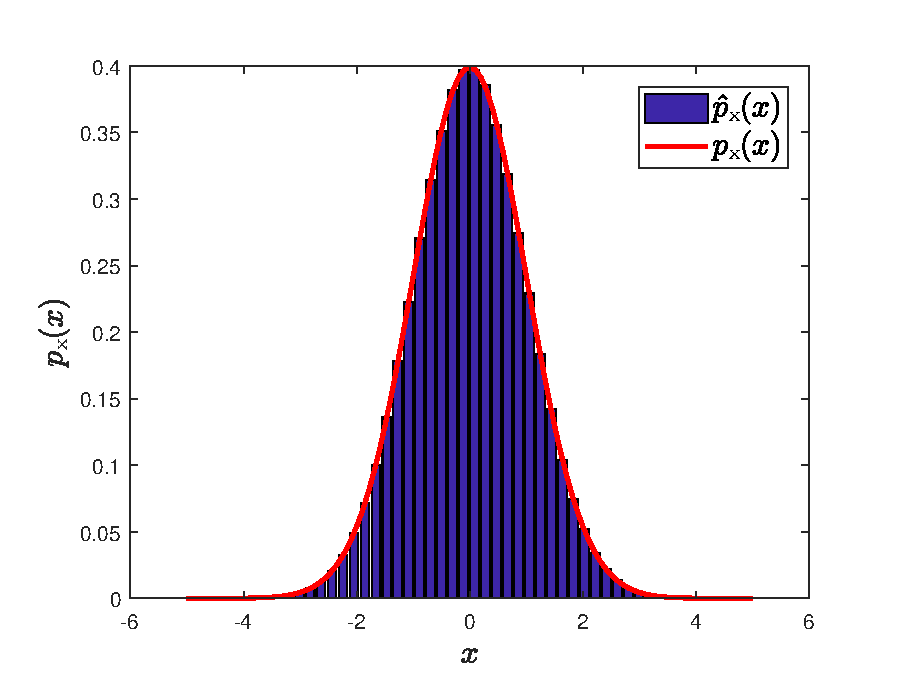
\includegraphics[width = 0.8\textwidth]{pdf_normal.eps}
%       \caption{Gaussian PDF and histogram of samples}
%       \label{fig:1}
%     \end{figure}

%   The source code to plot Figure \ref{fig:1} could be found in Appendix \ref{sec:a:code}. Here are the core codes:
%   \lstinputlisting[firstline=4,lastline=4, firstnumber=4]{matlabscript.m}
%   \lstinputlisting[firstline=6,lastline=7, firstnumber=6]{matlabscript.m}
%   To understand line 6, note that if we have $n$ samples of $X$ denoted by $x^{(i)}, i = 1, 2, \cdots, n$, then the probability density function $p_{X}$ can be estimated as
%   \begin{equation*}
%     \begin{aligned}
%       p_{X}(x_0) &= \left.\frac{\mathrm{d}}{\mathrm{d}x} \Prob(X \leq x) \right|_{x = x_0} \\
%       &\approx \frac{\Prob(x_0 - \Delta x < X \leq x_0)}{\Delta x}\\
%       &\approx \frac{1}{n\Delta x} \sum_{i = 1}^n \1_{x^{(i)} \in (x_0 - \Delta x, x_0]}.
%     \end{aligned}    
%   \end{equation*}
    
\end{enumerate}
  
  % \newpage
  
  % \appendix
  % \section{Source code}
  % \label{sec:a:code}
  % % \lstlistoflistings
  % The source code for plotting Figure \ref{fig:1} is shown as follows.
  % \lstinputlisting{matlabscript.m}
  
\end{document}
%%% Local Variables:
%%% mode: latex
%%% TeX-master: t
%%% End:
